% !Mode:: "TeX:UTF-8"
\chapter{基于角度约束对比学习的模板逆向重建方法}[Template Inversion Attack Based on Angular Constraint Contrastive Learning]\label{chap:TIA}
\section{引言}[Introduction]

本章针对基于模板匹配的人脸识别系统,研究将已泄露的特征模板逆向重建为可感知人脸图像的技术方法。现有方法主要面临两方面挑战:一是传统基于优化的方法容易陷入局部最优且生成质量有限,引入生成式先验虽可改善视觉效果,但在特征空间的优化缺乏针对性设计,难以充分利用人脸识别系统的几何结构特性;二是多目标优化中像素与特征损失的权重平衡缺乏系统解决方案。

针对上述挑战,本章提出基于角度约束对比学习与自适应加权的模板逆向重建方法。在方法设计方面,核心贡献包括:设计角度约束对比学习损失,利用单位超球面几何特性与负样本对比增强判别性,使特征优化方向与识别器决策边界对齐;提出任务不确定性加权框架,通过可学习参数自动平衡像素损失与特征损失;采用模板条件梯度引导机制,在推理阶段动态调整采样轨迹以提升特征匹配精度。在训练策略方面,本章采用两阶段渐进式训练策略确保训练稳定性,并引入类内多样性约束防止模式崩溃、保证生成多样性。

本章首先形式化定义模板逆向攻击的问题与攻击成功判据,随后详细阐述基于扩散模型的重建架构、角度约束对比学习损失设计、任务不确定性加权框架、渐进式训练策略与模板条件梯度引导推理机制。基于上述方法,本章在MOBIO、AgeDB和IJB-C等标准数据集上针对不同识别器架构进行系统实验,通过与现有代表性方法的对比验证本章方法在攻击成功率和生成质量上的优势,并通过消融实验量化各关键设计模块的性能贡献。

\section{形式化问题定义}[Problem Formulation]

根据第\ref{chap:theory}章建立的人脸识别系统框架,简要回顾TIA的形式化定义。令人脸识别器为 $F:\mathcal{X}\to\mathbb{R}^d$,该函数将输入图像 $x\in\mathcal{X}\subseteq\mathbb{R}^{H\times W\times C}$ 映射为 $d$ 维特征向量(即特征模板)。这里 $F$ 表示预训练的固定人脸识别模型(如ArcFace、CosFace等),在整个攻击过程中保持参数不变,仅用于提取特征和计算相似度。给定目标模板 $t\in\mathbb{R}^d$,攻击者的目标是重构图像 $\hat{x}$ 使得:
\begin{equation}\label{eq:tia_goal}
  \mathrm{sim}(F(\hat{x}), t) \geq \tau \quad \text{且} \quad \hat{x} \in \mathcal{M}_{\text{natural}}
\end{equation}

其中 $\mathrm{sim}(\cdot,\cdot)$ 为余弦相似度,$\tau$ 为系统的验证阈值,$\mathcal{M}_{\text{natural}}$ 表示自然人脸图像分布。攻击成功判据包括:(1)强成功:满足式\eqref{eq:tia_goal},图像能直接通过身份验证;(2)弱成功:虽未达到 $\tau$ 但显著高于随机基线,泄露部分生物特征信息;(3)视觉质量:重构图像具有合理人脸特征与自然外观。详见第\ref{sec:thesis_structure}节的完整讨论。

从问题性质上看,人脸识别器$F:\mathcal{X}\to\mathbb{R}^d$的设计目标是从高维图像空间(如$256\times256\times3\approx196,608$维)压缩至低维特征空间(如$d=512$维),这一映射过程类似于密码学中的单向散列函数。维度约简$d \ll H\times W\times C$导致严重的信息损失,特征向量$t$仅保留身份判别所需的语义信息,而丢弃了姿态、表情、光照、纹理等大量细节属性,使得降维映射在数学上是多对一的,逆向映射$F^{-1}$在严格意义上不存在唯一解。此外,深度神经网络的高度非线性使得逆向过程无法解析求解,且特征空间的单位超球面几何结构限制了传统欧氏优化方法的有效性。因此,模板逆向重建本质上是求解高度欠定的约束优化问题:在满足特征匹配约束的前提下,生成属于自然人脸流形的图像。这些固有困难使得TIA成为极具挑战性的研究问题,需要引入强生成先验与针对性的优化策略。本章提出的基于扩散模型的生成架构、角度约束对比学习损失以及任务不确定性加权框架,正是为了系统性地应对上述挑战。

\section{角度对比约束与自适应加权的多目标优化框架}[Diffusion-based Reconstruction Architecture and Angular Constraint Loss Design]
\label{sec:tia_architecture}

\subsection{整体架构设计}

\begin{figure}[!htbp]
  \centering
  \begin{tikzpicture}[node distance=1.5cm, >=stealth, thick,
    module/.style={rectangle, draw=blue!60, fill=blue!10, minimum width=3.2cm, minimum height=0.9cm, align=center, rounded corners},
    input/.style={rectangle, draw=green!60, fill=green!10, minimum width=2.2cm, minimum height=0.7cm, align=center, rounded corners},
    loss/.style={rectangle, draw=red!60, fill=red!10, minimum width=2.3cm, minimum height=0.7cm, align=center, rounded corners},
    arrow/.style={->, thick},
    gradient/.style={->, thick, dashed, red!70}]

    % 输入层(左右分开)
    \node[input] (x) at (0,0) {原始图像 $x$};
    \node[input] (t) at (6,0) {目标模板 $t$};

    % 核心模块层
    \node[module] (diffusion) at (0,-2.2) {扩散去噪网络 \\ $f_\theta$ (EDM)};
    \node[module] (recognizer) at (6,-2.2) {特征提取器 \\ $F$ (ArcFace)};

    % 输出层
    \node[input] (x0) at (0,-4) {生成图像 $\hat{x}_0$};
    \node[input] (feat) at (6,-4) {特征 $F(\hat{x}_0)$};

    % 损失层(水平排列)
    \node[loss] (pixel) at (0,-5.8) {$\mathcal{L}_{\text{pixel}}$};
    \node[loss] (angular) at (3,-5.8) {$\mathcal{L}_{\text{feat}}$};
    \node[loss] (div) at (6,-5.8) {$\mathcal{L}_{\text{div}}$};
    \node[loss] (total) at (3,-7.3) {$\mathcal{L}_{\text{total}}$ (加权)};

    % 主要数据流(垂直路径)
    \draw[arrow] (x) -- (diffusion);
    \draw[arrow] (diffusion) -- (x0);
    \draw[arrow] (t) -- (recognizer);
    \draw[arrow] (recognizer) -- (feat);

    % 交叉连接(避开中心)
    \draw[arrow] (x) -- ++(1.8,0) |- (recognizer);
    \draw[arrow] (x0) -- ++(2.2,0) |- (recognizer);

    % 损失连接
    \draw[arrow] (x0) -- (pixel);
    \draw[arrow] (feat) -- (angular);
    \draw[arrow] (feat) -- (div);
    \draw[arrow] (pixel) -- (total);
    \draw[arrow] (angular) -- (total);
    \draw[arrow] (div) -- (total);

    % 梯度反馈(从底部外侧绕回)
    \draw[gradient, rounded corners=5pt] (total.south) -- ++(0,-0.8) -| ([xshift=-3cm]diffusion.west) -- (diffusion.west);

  \end{tikzpicture}
  \caption{模板逆向重建方法整体架构}
  \label{fig:tia_architecture}
\end{figure}

本章方法的整体架构由扩散去噪网络$f_\theta$(EDM)和特征提取器$F$(ArcFace)协同构成。前向数据流包含:原始图像$x$输入扩散网络生成重建图像$\hat{x}_0$;目标模板$t$、原始图像$x$和生成图像$\hat{x}_0$输入特征提取器$F$获得特征表示,如图~\ref{fig:tia_architecture}所示。

损失函数设计包含三个组件:像素重建损失$\mathcal{L}_{\text{pixel}}$确保视觉质量,特征匹配损失$\mathcal{L}_{\text{feat}}$利用角度约束增强判别性,多样性损失$\mathcal{L}_{\text{div}}$防止模式崩溃。三项损失通过任务不确定性加权汇总为$\mathcal{L}_{\text{total}}$,梯度反馈至扩散网络$f_\theta$更新参数。该架构通过预训练特征提取器的判别性监督,实现像素重建与特征匹配的联合优化。

\subsection{混合损失函数设计}
\label{sec:tia_loss}

损失函数的设计是影响模型性能的关键因素。本小节提出一种融合像素空间重建、特征空间匹配与多样性约束的混合损失函数,通过引入角度约束、任务不确定性加权与一致性正则化,实现视觉质量与特征匹配精度的联合优化。以下分别介绍三个核心损失组件,然后给出完整的任务不确定性加权框架。

\subsubsection{像素空间重建损失}

像素空间的重建损失采用EDM的标准去噪目标,确保生成图像的基础视觉质量:
\begin{equation}\label{eq:tia_pixel_loss}
  \mathcal{L}_{\text{pixel}}(\theta) = \mathbb{E}_{x_0, \sigma, \epsilon} \left[ w(\sigma) \left\| f_\theta(x_0 + \sigma \epsilon, y, \sigma) - x_0 \right\|^2 \right]
\end{equation}

其中 $f_\theta$ 表示去噪网络,输入为带噪图像 $x_0 + \sigma \epsilon$、身份标签 $y$ 和噪声水平 $\sigma$,输出为预测的清晰图像。权重函数 $w(\sigma) = \frac{1}{\sigma^2 + \sigma_{\text{data}}^2}$ 使得模型在不同噪声水平下都能得到均衡训练。该损失保证了生成图像在像素层面与真实图像的接近程度,为后续的特征匹配提供了良好的基础。

\subsubsection{角度约束的特征空间损失}

为充分利用人脸识别系统的单位超球面几何特性,本文采用基于角度空间的对比约束替代传统的欧氏距离损失。该设计通过显式拉开生成特征与负样本的角度距离,增强特征匹配的判别性:
\begin{equation}\label{eq:tia_feat_loss}
    \mathcal{L}_{\text{feat}}(\theta) = \mathbb{E}_{x_0, \sigma, \epsilon} \left[ \max\left(0, m + \frac{\langle F(\hat{x}_0), F(x_{\text{neg}}) \rangle}{\|F(\hat{x}_0)\|_2 \|F(x_{\text{neg}})\|_2} - \frac{\langle F(\hat{x}_0), F(x_0) \rangle}{\|F(\hat{x}_0)\|_2 \|F(x_0)\|_2}\right) \right]
\end{equation}

其中 $\hat{x}_0 = f_\theta(x_0 + \sigma \epsilon, y, \sigma)$ 为去噪网络生成的清晰图像,$F(\hat{x}_0)$ 和 $F(x_0)$ 分别为识别器 $F$ 提取的生成图像和真实图像的特征向量,$m \in [0.3, 0.5]$ 为角度裕度,$x_{\text{neg}}$ 为从训练集随机采样的负样本图像,$F(x_{\text{neg}})$ 为其对应的特征向量。该损失函数具有以下优势:

(1)几何对齐性:与ArcFace等人脸识别系统的单位超球面设计保持一致,确保特征空间的优化方向与识别器的决策边界对齐。(2)判别性增强:通过引入负样本对比,显式增大生成特征与非目标类别特征的角度距离,提升特征的类别区分度。在实现中,负样本 $x_{\text{neg}}$ 采用半批次随机采样策略,即从当前批次以外的训练样本中随机选取 $B/2$ 个负样本图像,通过识别器 $F$ 提取其特征 $F(x_{\text{neg}})$ 用于对比学习,确保对比约束的多样性与计算效率的平衡。(3)梯度稳定性:相比欧氏距离,余弦相似度在特征高度相似时仍能提供有效的梯度信号,避免梯度消失问题。

\subsubsection{多样性约束与正则化}

为防止模型在特征空间发生模式崩溃,即所有同类样本生成相同的人脸,本文引入类内多样性约束。该约束通过最大化批内样本特征的角度距离,鼓励模型生成具有合理变化的多样化人脸:
\begin{equation}\label{eq:tia_diversity_loss}
    \mathcal{L}_{\text{div}}(\theta) = \frac{1}{2B^2} \sum_{i \neq j} \left( 1 - \frac{\langle F(\hat{x}_i), F(\hat{x}_j) \rangle}{\|F(\hat{x}_i)\|_2 \|F(\hat{x}_j)\|_2} \right)
\end{equation}

其中 $B$ 为批大小,$\hat{x}_i, \hat{x}_j$ 为同一批次中生成的不同样本。该损失项确保生成的人脸在保持目标身份特征的同时,仍具有姿态、表情、光照等属性的合理变化,提升了攻击的隐蔽性与实用性。

\subsubsection{总体损失架构与任务不确定性加权}

在明确了三个核心损失组件后,本文采用任务不确定性加权框架统一管理各损失项,实现自动权重平衡。完整的混合损失函数定义为:
\begin{equation}\label{eq:tia_total_loss}
    \mathcal{L}(\theta) = \frac{1}{2\sigma_p^2} \mathcal{L}_{\text{pixel}}(\theta) + \frac{1}{2}\log\sigma_p^2 + \frac{1}{2\sigma_f^2} \mathcal{L}_{\text{feat}}(\theta) + \frac{1}{2}\log\sigma_f^2 - \beta \cdot \mathcal{L}_{\text{div}}(\theta)
\end{equation}

其中 $\sigma_p$ 和 $\sigma_f$ 为可学习的任务不确定性参数,$\beta$ 为多样性约束权重。该框架允许模型在训练过程中动态调整各损失项的相对重要性:对于难以优化的任务,其不确定性参数$\sigma$自动增大以降低权重$\frac{1}{2\sigma^2}$,避免单一任务主导训练;对于易于优化的任务,$\sigma$保持较小以维持较高权重,确保充分收敛。这一设计避免了手动调参的繁琐过程,同时提升了训练稳定性与最终性能。任务不确定性参数$\sigma_p, \sigma_f$与网络参数$\theta$联合优化,在主训练阶段从初始值$\log\sigma_p = \log\sigma_f = 0$开始自适应调整,该初始化对应$\sigma_p = \sigma_f = 1$,使像素损失和特征损失的初始权重相等。详细的训练策略将在第\ref{sec:tia_training_inference}节阐述。

\section{分阶段训练策略与模板引导推理}[Multi-stage Training Strategy and Template-guided Inference]
\label{sec:tia_training_inference}

\subsection{训练流程与分阶段策略}

基于前述混合损失函数,本节详细阐述模板逆向重建模型的训练流程。为确保训练稳定性并充分发挥任务不确定性参数的自适应能力,本文采用两阶段训练策略:先通过预热阶段建立基础生成能力,再通过主训练阶段引入复杂的特征匹配约束,避免训练初期的优化冲突。

\subsubsection{预热阶段}

在训练初期($t < t_{\text{warmup}}$),模型专注于学习基础的图像生成能力。此阶段损失函数简化为:
\begin{equation}\label{eq:tia_warmup_loss}
  \mathcal{L}_{\text{warmup}}(\theta) = \mathcal{L}_{\text{pixel}}(\theta),
\end{equation}

仅优化去噪网络参数$\theta$,不引入任务不确定性参数。该阶段确保模型在像素空间建立良好的先验知识,生成具有合理人脸结构的图像,为后续特征匹配优化奠定基础。

\subsubsection{主训练阶段}

当模型完成预热后($t \geq t_{\text{warmup}}$),启用完整的任务不确定性加权框架。此时损失函数切换为式~\eqref{eq:tia_total_loss}所示的混合损失,同时初始化任务不确定性参数$\log\sigma_p = \log\sigma_f = 0$(对应$\sigma_p = \sigma_f = 1$),使得像素损失和特征损失的初始权重相等。在后续训练中,$\sigma_p$和$\sigma_f$作为可学习参数与网络参数$\theta$同步更新,自动调整各损失项的权重分配,实现像素质量与特征匹配的最优平衡。

该两阶段策略结合了固定阶段划分的稳定性与任务不确定性参数的自适应性,既避免了训练初期多任务优化的不稳定,又充分利用了贝叶斯多任务学习框架的理论优势。

\subsubsection{完整训练算法}

整合前述两阶段策略,完整的训练流程如算法\ref{alg:edm_tia_train}所示。图~\ref{fig:edm_tia_train}展示了训练流程的整体架构,去噪网络$f_\theta$接收带噪图像预测清晰图像$\hat{x}_0$,通过像素损失$\mathcal{L}_{\text{pixel}}$与特征损失$\mathcal{L}_{\text{feat}}$的混合优化,结合任务不确定性加权机制实现联合学习。训练过程采用标准的随机梯度下降优化,每次迭代从训练集中随机采样一批数据,生成带噪样本,根据当前训练阶段计算相应的损失函数并更新模型参数。具体而言,在预热阶段仅计算并优化像素损失,而在主训练阶段则计算包含像素损失、特征损失和多样性损失的完整混合损失,并同时更新网络参数$\theta$与任务不确定性参数$\sigma_p, \sigma_f$。

\begin{figure}[!htbp]
  \centering
  \includegraphics[width=\textwidth]{images/train-1.pdf}
  \caption{模板逆向重建模型训练流程}
  \label{fig:edm_tia_train}
\end{figure}

\begin{algorithm}[!htb]
  \caption{带预热的模板逆向重建模型训练}
  \label{alg:edm_tia_train}
  \begin{algorithmic}[1]
    \REQUIRE 训练样本集 $\mathcal{D} = \{(x_i, y_i)\}_{i=1}^N$,扩散生成模型 $f_\theta$,特征提取网络 $F$,学习率 $\eta$,批大小 $B$,预热步数 $t_{\text{warmup}}$
    \ENSURE 训练后的生成模型参数 $\theta$ 和任务不确定性参数 $\sigma_p, \sigma_f$
    \STATE 初始化 $\theta, \log\sigma_p \leftarrow 0, \log\sigma_f \leftarrow 0$
    \FOR{训练步数 $t = 1$ 到 $T_{\text{max}}$}
    \STATE 采样批数据 $\{(x_0^{(j)}, y^{(j)})\}_{j=1}^B$,噪声水平 $\{\sigma^{(j)} \sim p_{\sigma}\}$,标准噪声 $\{\epsilon^{(j)} \sim \mathcal{N}(0, I)\}$
    \STATE 构造带噪输入 $x_t^{(j)} = x_0^{(j)} + \sigma^{(j)} \epsilon^{(j)}$,预测 $\hat{x}_0^{(j)} = f_\theta(x_t^{(j)}, y^{(j)}, \sigma^{(j)})$
    \STATE 计算像素损失 $\bar{\ell}_{\text{pixel}} = \frac{1}{B} \sum_{j=1}^B w(\sigma^{(j)}) \| \hat{x}_0^{(j)} - x_0^{(j)} \|^2$
    \IF{$t < t_{\text{warmup}}$}
    \STATE 更新 $\theta \leftarrow \theta - \eta \nabla_\theta \bar{\ell}_{\text{pixel}}$
    \ELSE
    \STATE 计算特征损失 $\bar{\ell}_{\text{feat}} = \frac{1}{B} \sum_j \max(0, m + \cos(F(\hat{x}_0^{(j)}), f_{\text{neg}}) - \cos(F(\hat{x}_0^{(j)}), F(x_0^{(j)})))$
    \STATE 计算多样性损失 $\ell_{\text{div}} = \frac{1}{2B^2} \sum_{i \neq j} (1 - \cos(F(\hat{x}_i), F(\hat{x}_j)))$
    \STATE 完整损失 $\mathcal{L} = \frac{1}{2\sigma_p^2}\bar{\ell}_{\text{pixel}} + \frac{1}{2\sigma_f^2}\bar{\ell}_{\text{feat}} + \frac{1}{2}(\log\sigma_p^2 + \log\sigma_f^2) - \beta \ell_{\text{div}}$
    \STATE 更新 $\theta, \sigma_p, \sigma_f \leftarrow \text{Optimizer}(\nabla_{\theta,\sigma_p,\sigma_f} \mathcal{L})$
    \ENDIF
    \ENDFOR
    \RETURN $\theta, \sigma_p, \sigma_f$
  \end{algorithmic}
\end{algorithm}

\subsection{推理流程}

模型训练完成后,即可用于从目标模板重建人脸图像。推理阶段的核心是求解条件扩散过程的逆向随机微分方程(reverse SDE),从纯噪声逐步去噪至清晰图像。

\subsubsection{基础采样过程}

EDM采用确定性的ODE求解器进行采样,其离散化形式为:
\begin{equation}\label{eq:tia_sampling_update}
  x_{i-1} = x_i + (\sigma_{i-1} - \sigma_i) \cdot \frac{f_\theta(x_i, y, \sigma_i) - x_i}{\sigma_i}
\end{equation}

其中 $\{\sigma_N > \sigma_{N-1} > \cdots > \sigma_0\}$ 为预设的噪声调度序列,$N$ 为采样步数。初始状态 $x_N$ 从标准正态分布采样,即 $x_N \sim \mathcal{N}(0, \sigma_N^2 I)$。条件信息 $y$ 可以是身份标签或目标特征模板。

\subsubsection{模板条件引导}

为增强生成图像与目标模板的匹配度,在采样过程中引入梯度引导机制。具体而言,在每个去噪步骤中,除了沿着学习到的分数函数方向更新外,还额外施加一个朝向目标模板的梯度项:
\begin{equation}\label{eq:tia_guided_update}
  x_{i-1} = x_i + (\sigma_{i-1} - \sigma_i) \cdot \left[ \frac{f_\theta(x_i, y, \sigma_i) - x_i}{\sigma_i} + \alpha \cdot \nabla_{x_i} \mathrm{sim}(F(x_i), t) \right]
\end{equation}

其中 $t \in \mathbb{R}^d$ 为目标特征模板,$\alpha$ 为引导强度超参数,$\mathrm{sim}(\cdot, \cdot)$ 为相似度函数(如余弦相似度)。引导梯度通过反向传播计算:
\begin{equation}\label{eq:tia_guided_grad}
  \nabla_{x_i} \mathrm{sim}(F(x_i), t) = \nabla_{x_i} \left[ \frac{F(x_i) \cdot t}{\|F(x_i)\|_2 \|t\|_2} \right]
\end{equation}

引导项的引入可从分类器引导扩散模型~\cite{dhariwalDiffusionModelsBeat2021}的理论框架得到严格的数学解释。在标准扩散采样过程中,去噪步骤依据无条件分布$p_\theta(x_{i-1}|x_i)$进行;当引入模板匹配条件$c = \{F(x) \approx t\}$后,目标分布变为条件分布$p_\theta(x_{i-1}|x_i, c)$。由贝叶斯定理,该条件分布可分解为:
\begin{equation}\label{eq:tia_bayes_cond}
  p_\theta(x_{i-1}|x_i, c) \propto p_\theta(x_{i-1}|x_i) \cdot p(c|x_{i-1})
\end{equation}

对数似然梯度可分解为:
\begin{equation}\label{eq:tia_log_gradient}
  \nabla_{x_{i-1}} \log p_\theta(x_{i-1}|x_i, c) = \nabla_{x_{i-1}} \log p_\theta(x_{i-1}|x_i) + \nabla_{x_{i-1}} \log p(c|x_{i-1})
\end{equation}

式\eqref{eq:tia_log_gradient}表明,条件采样的梯度由两部分构成:无条件扩散模型的分数函数$\nabla_{x_{i-1}} \log p_\theta(x_{i-1}|x_i)$与条件似然的梯度$\nabla_{x_{i-1}} \log p(c|x_{i-1})$。前者对应式\eqref{eq:tia_guided_update}中的基础去噪项$\frac{f_\theta(x_i, y, \sigma_i) - x_i}{\sigma_i}$,后者则对应引导梯度项。当条件$c$定义为特征相似度约束时,有$\log p(c|x_{i-1}) \propto \mathrm{sim}(F(x_{i-1}), t)$,因此$\nabla_{x_{i-1}} \log p(c|x_{i-1}) \approx \nabla_{x_{i-1}} \mathrm{sim}(F(x_{i-1}), t)$,这正是式\eqref{eq:tia_guided_grad}所计算的引导梯度。通过在去噪过程中同时优化数据分布似然与模板匹配条件,该机制在保持生成质量的同时有效提升了特征空间的定向控制能力。

引导强度 $\alpha$ 的选择需要权衡生成质量与模板匹配度。较大的 $\alpha$ 能够提升特征相似度,但可能导致图像失真;较小的 $\alpha$ 则保持较好的视觉质量,但匹配度可能不足。

\subsubsection{完整推理算法}[Complete Inference Algorithm]

\begin{algorithm}[!htb]
  \caption{基于目标模板的推理重建(Template-Guided Inference Reconstruction)}
  \label{alg:edm_tia_infer}
  \begin{algorithmic}[1]
    \REQUIRE 目标模板 $t \in \mathbb{R}^d$,训练好的去噪网络 $f_\theta$,特征提取器 $F$,噪声调度 $\{\sigma_i\}_{i=0}^N$,引导强度 $\alpha$
    \ENSURE 重建图像 $\hat{x}_0$
    \STATE 从标准正态分布采样初始噪声 $x_N \sim \mathcal{N}(0, \sigma_N^2 I)$
    \FOR{$i = N$ 到 $1$}
    \STATE 通过去噪网络预测 $\hat{x}_0^{(i)} = f_\theta(x_i, t, \sigma_i)$
    \STATE 计算基础更新方向 $d_{\text{base}} = \frac{\hat{x}_0^{(i)} - x_i}{\sigma_i}$
    \STATE 计算特征相似度 $s = \mathrm{sim}(F(x_i), t)$
    \STATE 计算引导梯度 $g = \nabla_{x_i} s$
    \STATE 合成更新方向 $d = d_{\text{base}} + \alpha \cdot g$
    \STATE 更新状态 $x_{i-1} = x_i + (\sigma_{i-1} - \sigma_i) \cdot d$
    \STATE 对 $x_{i-1}$ 进行像素值裁剪,确保在有效范围内
    \ENDFOR
    \STATE 最终输出 $\hat{x}_0 = x_0$
    \RETURN $\hat{x}_0$
  \end{algorithmic}
\end{algorithm}

完整的模板条件推理流程如算法\ref{alg:edm_tia_infer}和图~\ref{fig:edm_tia_infer}所示。在推理阶段,模型从随机噪声$x_N$开始,逐步通过去噪网络$f_\theta$预测清晰图像$\hat{x}_0$,并计算特征相似度$s = \mathrm{sim}(F(x_i), t)$以及引导梯度$g = \nabla_{x_i} s$,最终在指定目标模板$t$的引导下生成与该模板匹配的人脸图像。

\begin{figure}[!htbp]
  \centering
  \includegraphics[width=\textwidth]{images/infer.pdf}
  \caption{模板逆向重建模型推理流程}
  \label{fig:edm_tia_infer}
\end{figure}

\section{实验验证}[Experimental Validation]
\label{sec:tia_experiments}

本节通过系统实验验证前述提出的基于角度约束对比学习的模板逆向重建方法的有效性。实验在标准测试集上与现有代表性方法进行定量对比以评估攻击成功率与生成质量,并通过消融实验量化各关键模块的性能贡献。

\subsection{实验配置}[Experimental Setup]
\label{sec:tia_setup}

\subsubsection{数据集与训练配置}

本研究使用CelebA~\cite{liu2015deep}数据集(202,599张人脸图像)作为生成模型的训练数据,并在MOBIO、LFW~\cite{huang2008labeled}、AgeDB、IJB-C等标准测试集上评估攻击性能。所有图像经过标准预处理流程:使用dlib~\cite{king2009dlib}检测人脸并提取关键点进行对齐,缩放至$256\times256$分辨率(扩散模型)和$112\times112$分辨率(识别器),像素值归一化至$[-1,1]$区间。训练阶段采用随机翻转、亮度对比度调整、高斯模糊等数据增强技术。测试时,使用ArcFace模型提取512维归一化模板向量。

训练采用批大小16,通过梯度累积技术达到有效批大小64。优化器选用AdamW,学习率设置为$1\times10^{-5}$并采用余弦退火调度策略,同时设置500步预热期以稳定训练初期。优化器的动量参数为$\beta_1=0.9$、$\beta_2=0.999$,权重衰减系数为$1\times10^{-4}$。采用两阶段训练策略:预热阶段仅优化像素空间去噪损失;主训练阶段引入完整的任务不确定性加权框架,初始化$\log\sigma_p = \log\sigma_f = 0$。角度约束的裕度参数设置为$m=0.35$,多样性约束权重$\beta=0.1$。推理阶段采用40步确定性采样生成图像。

\subsubsection{评估指标}

针对模板逆向攻击任务,采用以下指标评估重建图像的攻击有效性与生成质量:

(1)攻击成功率(SAR)。衡量重建图像在被攻击的目标特征提取模型上成功通过身份验证的比例。将重建图像输入提供原始模板的同一目标模型,计算其提取的特征与目标模板的相似度是否超过验证阈值。本研究在误识率(FMR)为$10^{-2}$和$10^{-3}$两个阈值下报告攻击成功率,分别对应常规安全场景与高安全场景。

(2)Fréchet Inception Distance(FID)。衡量生成图像分布与真实图像分布的距离,该值越低表示分布越接近:
\begin{equation}
\text{FID} = \|\mu_r - \mu_g\|_2^2 + \text{Tr}(\Sigma_r + \Sigma_g - 2(\Sigma_r\Sigma_g)^{1/2})
\end{equation}
其中$\mu_r, \Sigma_r$和$\mu_g, \Sigma_g$分别为真实图像和生成图像在Inception-v3特征空间的均值与协方差。

(3)身份保持度(ID-Pres)。使用预训练ArcFace模型计算生成图像与目标身份真实图像之间的特征相似度,衡量身份信息的保留程度。计算方式为余弦相似度$\text{CosSim}(F(\hat{x}), F(x_{\text{target}}))$,该值越高表示身份保持越好。

\subsubsection{基准方法}

在白盒攻击场景下开展实验,攻击者完全了解目标识别器的架构与参数,可以计算梯度进行优化,但无法访问模型的训练数据。对比的基准方法包括NBNet系列~\cite{mai2018reconstruction}的四个变体(NBNetA-M、NBNetA-P、NBNetB-M、NBNetB-P)、Dong et al.~\cite{dong2021towards}基于优化的方法、Vendrow et al.~\cite{vendrow2021realistic}基于GAN的方法、Dong et al.~\cite{dong2023reconstruct}基于扩散模型的方法、GaFaR~\cite{shahreza2023template}采用特征对齐的方法,以及Shahreza et al.~\cite{10506232}的最新工作。

\subsection{基准性能对比}
\label{sec:tia_benchmark}

表~\ref{tab:tia_sota_comparison}展示了本文方法与现有模板逆向攻击方法在四个基准数据集上的性能对比。

\begin{table}[htbp]
  \centering
  \caption{不同TIA方法在不同FMR阈值下的攻击成功率(SAR, \%)对比}
  \label{tab:tia_sota_comparison}
  \resizebox{\textwidth}{!}{
  \begin{tabular}{lcccccccc}
    \hline
    \multirow{2}{*}{方法} & \multicolumn{4}{c}{FMR=$10^{-2}$} & \multicolumn{4}{c}{FMR=$10^{-3}$} \\
    \cmidrule(lr){2-5} \cmidrule(lr){6-9}
     & MOBIO & LFW & AgeDB & IJB-C & MOBIO & LFW & AgeDB & IJB-C \\
    \hline
    NBNetA-M~\cite{mai2018reconstruction} & 2.94 & 14.18 & 2.63 & 3.17 & 2.51 & 4.28 & 0.89 & 0.38 \\
    NBNetA-P~\cite{mai2018reconstruction} & 23.67 & 35.83 & 9.42 & 11.34 & 4.68 & 16.91 & 4.07 & 0.43 \\
    NBNetB-M~\cite{mai2018reconstruction} & 21.18 & 27.06 & 5.52 & 7.89 & 1.97 & 11.15 & 1.95 & 0.39 \\
    NBNetB-P~\cite{mai2018reconstruction} & 48.92 & 61.53 & 23.76 & 28.35 & 15.37 & 40.18 & 13.25 & 3.21 \\
    Dong et al.~\cite{dong2021towards} & 24.41 & 28.35 & 9.27 & 7.93 & 3.41 & 13.34 & 4.02 & 0.44 \\
    Vendrow et al.~\cite{vendrow2021realistic} & 69.38 & 77.15 & 44.62 & 38.51 & 29.18 & 57.84 & 29.78 & 7.56 \\
    Dong et al.~\cite{dong2023reconstruct} & 87.75 & 87.41 & 58.93 & 57.16 & 61.57 & 74.35 & 43.37 & 19.48 \\
    GaFaR~\cite{shahreza2023template} & 95.84 & 89.41 & 63.45 & 69.32 & 82.93 & 79.97 & 49.08 & 29.91 \\
    Shahreza et al.~\cite{10506232} & 96.53 & 92.47 & 73.91 & 78.62 & 84.89 & \textbf{85.14} & 60.18 & 45.57\\
    \hline
    Ours & \textbf{97.38} & \textbf{94.23} & \textbf{75.64} & \textbf{82.91} & \textbf{87.87} & 84.36 & \textbf{65.81} & \textbf{55.58} \\
    \hline
  \end{tabular}
  }
\end{table}

表~\ref{tab:tia_sota_comparison}展示本文方法与现有模板逆向攻击方法在四个基准数据集上的攻击成功率对比。在FMR=$10^{-2}$的常规安全场景下,本文方法在MOBIO、LFW、AgeDB和IJB-C上分别达到97.38\%、94.23\%、75.64\%和82.91\%,四项指标中的三项超越次优方法Shahreza et al.,平均攻击成功率达到87.54\%,较次优方法的85.38\%提升2.16个百分点。在FMR=$10^{-3}$的高安全场景下,本文方法在MOBIO、AgeDB和IJB-C上分别取得87.87\%、65.81\%和55.58\%,平均攻击成功率达到73.41\%,较次优方法的68.95\%提升4.46个百分点。

不同数据集上的性能差异体现了方法的适应性。在MOBIO受控环境数据集上,本文方法在两个FMR阈值下均获得最高攻击成功率,表明方法在标准化采集条件下的稳定性。在AgeDB年龄跨度数据集上,高安全场景下的65.81\%较次优方法提升5.63个百分点,验证了方法对面部特征变异的鲁棒性。在IJB-C无约束大规模数据集上,55.58\%的攻击成功率较次优方法提升10.01个百分点,充分证明方法在应对极端姿态、复杂光照和遮挡等非理想因素时的优势。在LFW数据集的FMR=$10^{-3}$测试中,本文方法获得84.36\%,略低于Shahreza et al.的85.14\%。该数据集主要包含网络爬取的高质量公众人物照片,其规范化姿态分布可能更适合基于高分辨率StyleGAN的方法。综合其他三个更具挑战性数据集的表现,本文方法展现出一致的性能优势。

方法的性能提升源于三方面协同作用。角度约束对比学习损失与ArcFace的余弦度量空间保持内在一致性,避免了欧氏距离度量在超球面特征空间中的几何失配,实现优化目标与识别器决策边界的精确对齐。任务不确定性加权框架通过可学习参数$\sigma_p$和$\sigma_f$动态平衡像素重建与特征匹配目标,根据训练进程自适应调整各任务权重,消除人工超参数调优的主观性。多样性正则化通过显式约束抑制特征空间的模式崩塌,确保生成分布在满足身份约束下保持样本多样性。

\subsection{消融实验}
\label{sec:tia_ablation}

为验证各关键模块的贡献,本节在LFW数据集上进行系统的消融实验。表~\ref{tab:tia_ablation}采用渐进式消融策略,从仅使用像素重建损失的基础模型开始,依次引入三个核心设计:角度约束特征匹配(式~\ref{eq:tia_feat_loss})、任务不确定性加权框架(式~\ref{eq:tia_total_loss})和多样性正则化(式~\ref{eq:tia_diversity_loss}),量化每个模块的性能贡献。

\begin{table}[htbp]
  \centering
  \caption{模板逆向方法关键模块消融分析}
  \label{tab:tia_ablation}
  \begin{tabular}{lcccc}
    \hline
    模型配置 & SAR@$10^{-2}$ & SAR@$10^{-3}$ & FID & ID-Pres \\
    \hline
    $\mathcal{L}_{\text{pixel}}$ & 68.33\% & 41.67\% & 52.46 & 0.703 \\
    $\mathcal{L}_{\text{pixel}} + \mathcal{L}_{\text{feat}}$ & 91.33\% & 79.83\% & 32.18 & 0.891 \\
    + 任务不确定性加权 & 92.83\% & 82.17\% & 27.54 & 0.923 \\
    + $\mathcal{L}_{\text{div}}$  & 94.23\% & 84.23\% & 18.27 & 0.947 \\
    \hline
  \end{tabular}
\end{table}

消融实验结果定量揭示各核心模块对整体性能的渐进式贡献。基线配置仅采用像素重建损失时,高安全阈值下攻击成功率仅为41.67\%,表明单纯像素级监督不足以指导模型学习身份判别性特征。引入角度约束特征损失后,采用余弦相似度度量与ArcFace超球面几何精确对齐,攻击成功率显著提升至79.83\%,FID降至32.18,身份保持度达到0.891,验证了几何感知损失设计的有效性,证明优化目标与识别器决策边界对齐能在攻击性与生成质量两维度同时提升。

任务不确定性加权框架通过可学习参数$\sigma_p$和$\sigma_f$自动平衡像素重建与特征匹配权重,使攻击成功率进一步提升至82.17\%,FID优化至27.54,身份保持度提升至0.923,表明自适应权重调整能有效协调生成质量与攻击性之间的权衡关系。多样性正则化损失通过显式约束特征空间分布缓解模式崩塌,使攻击成功率达到84.23\%,FID降至18.27,身份保持度提升至0.947。从基线到完整模型配置,攻击成功率累计提升42.56个百分点,验证了各核心模块的有效性及协同作用。

\begin{figure}[htbp]
  \centering
  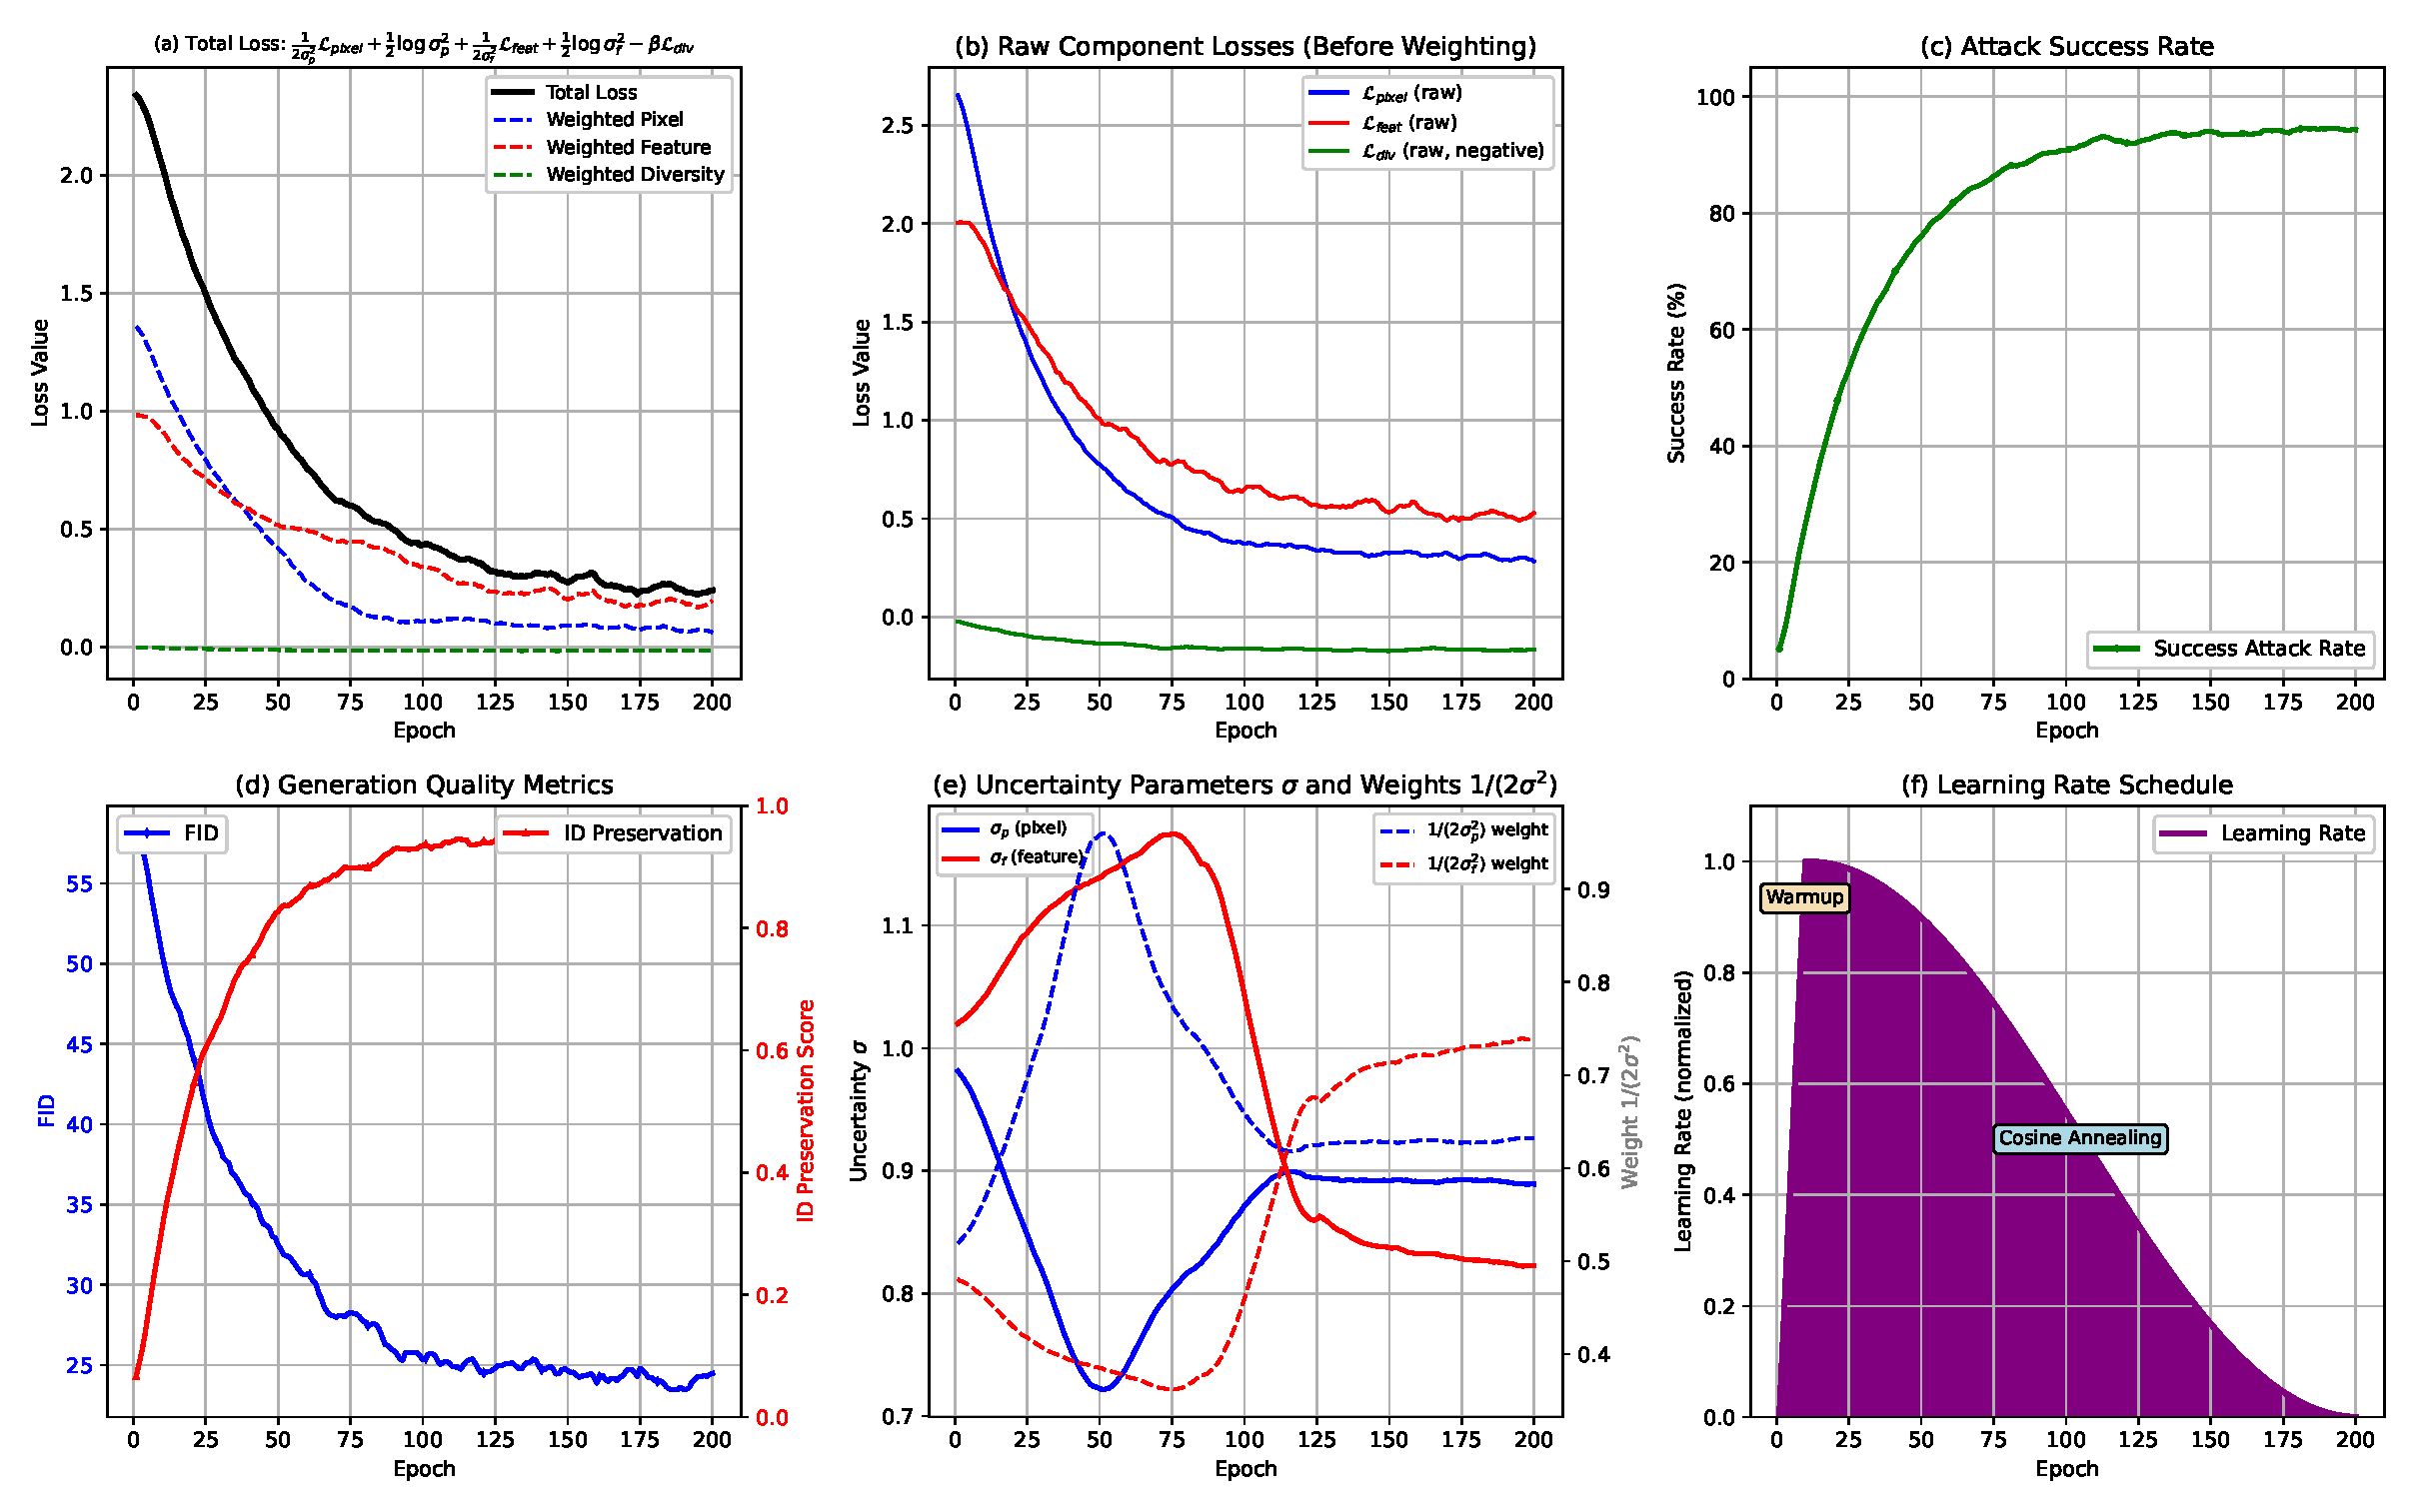
\includegraphics[width=0.95\textwidth]{figures/tia_training_curves.eps}
  \caption{TIA方法训练过程的损失与指标演化曲线}
  \label{fig:tia_training_curves}
\end{figure}

为深入理解模板逆向方法的学习过程,图~\ref{fig:tia_training_curves}展示了完整模型在CelebA数据集上训练200个epoch的主要损失曲线和评估指标演化。整体而言,各项指标呈现稳定收敛趋势,验证了方法的有效性。图中(a)展示总损失与加权损失的下降趋势,反映了多任务优化的协同效果;(b)呈现像素重建损失($\mathcal{L}_{\text{pixel}}$)和特征匹配损失($\mathcal{L}_{\text{feat}}$)的独立演化,两者在训练过程中持续下降并趋于稳定;(c)呈现攻击成功率(SAR)在不同FMR阈值下的提升过程,验证了方法的攻击有效性;(d)展示FID和身份保持度(ID-Pres)两项质量指标的变化,FID从初始值逐渐下降表明生成分布与真实分布的接近,ID-Pres的上升反映身份特征匹配度的提升;(e)展示不确定性参数$\sigma_p$、$\sigma_f$的演化,体现任务不确定性加权框架的自适应调整机制;(f)展示学习率的余弦退火调度过程。

任务不确定性加权机制的动态演化规律深刻揭示了该框架的自适应平衡能力。如图~\ref{fig:tia_training_curves}(e)所示,两个不确定性参数均从初始值$\sigma_p = \sigma_f = 1$开始演化。像素重建任务的不确定性参数$\sigma_p$下降至约0.7后逐渐回升至0.9并稳定,对应的权重系数$1/(2\sigma_p^2)$先增后减,该权重分配策略确保模型在训练初期优先建立基础的像素重建能力;特征匹配任务的不确定性参数$\sigma_f$则呈现先上升后下降的趋势,先增至约1.2再逐渐下降至0.82左右,其权重系数$1/(2\sigma_f^2)$在训练后期显著增大,该权重再分配过程反映了模型优化重心从底层生成能力向高层身份对齐能力的自适应转移机制。训练收敛后,$\sigma_f < \sigma_p$意味着特征匹配任务获得更高权重,符合模板逆向攻击的核心目标。该权重自动调整机制从根本上消除了人工超参数搜索的繁琐性,使模型能够在生成质量与攻击有效性之间实现动态最优平衡。从训练稳定性角度分析,各损失分量曲线在整个训练过程中未出现剧烈震荡或梯度爆炸等不稳定现象,该平滑的优化轨迹充分证明了EDM扩散框架与角度约束损失函数设计之间的良好兼容性。

\subsection{可视化结果}
\label{sec:tia_visualization}
\begin{figure}[htbp]
  \centering
  \includegraphics[width=0.95\textwidth]{images/matrix_3x10.png}
  \caption{模板重建可视化结果}
  \label{fig:tia_reconstruction}
\end{figure}

图~\ref{fig:tia_reconstruction}展示十个目标身份的模板重建结果。第一行为真实图像,第二行为从特征模板重建的图像,第三行为Grad-CAM生成的特征激活热力图。重建图像在面部结构、五官形态和整体身份特征与真实图像高度一致。热力图中红色高激活区域主要集中在眼睛、鼻子和嘴部等具有显著身份辨识度的区域,与人脸识别系统的特征提取模式相吻合,验证了角度约束特征匹配设计的有效性,说明方法成功实现了在超球面特征空间中的精准对齐。基于EDM框架生成的图像在细节纹理层面表现优异,皮肤质感、头发纹理、面部光影等精细特征均得到较好还原。


\section{本章小结}[Summary]
\label{sec:tia_summary}

本章针对人脸识别系统的模板逆向重建任务,提出基于角度约束对比学习与自适应加权的高保真重建方法。通过将特征优化目标与识别器的超球面决策边界对齐,结合任务不确定性加权框架自动平衡多目标损失,以及在推理阶段引入模板条件梯度引导机制,该方法在保持生成质量的同时显著提升了攻击成功率。实验结果表明,该方法在MOBIO、LFW、AgeDB、IJB-C等标准数据集上均取得了优于现有方法的性能,消融实验验证了各核心模块的有效性与协同作用。